\begin{figure}[!ht]
\subfigure[{}]{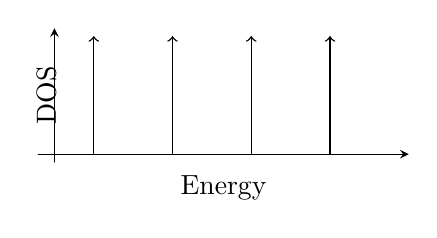
\begin{tikzpicture}[line cap=round,line join=round]
	\definecolor{grannysmithapple}{rgb}{0.66, 0.89, 0.63}
	\definecolor{unitednationsblue}{rgb}{0.36, 0.57, 0.9}
	\begin{axis}[ticks=none,
		x=1cm,y=1cm,
		axis lines=middle,
		xmin=-0.2052410812264766,
		xmax=4.5,ymin=-0.1,x label style={at={(axis description cs:0.5,-0.03)},anchor=north}, y label style={at={(axis description cs:-0.03,0.5)},rotate=90},
		ymax=1.6,xlabel=Energy,ylabel=DOS]
		\draw [->,line width=0.5pt] (0.5,0) -- (0.5,1.5);
		\draw [->,line width=0.5pt] (1.5,0) -- (1.5,1.5);
		\draw [->,line width=0.5pt] (2.5,0) -- (2.5,1.5);
		\draw [->,line width=0.5pt] (3.5,0) -- (3.5,1.5);
	\end{axis}
	\end{tikzpicture}}
	
\caption{The density of electron as decrease the magnetic field}
\end{figure}